\documentclass[a4paper, 11pt]{article}
%\usepackage[left=1in,right=1in,top=1in,bottom=1in]{geometry}
\usepackage[left=2cm,right=2cm,top=2cm,bottom=2cm]{geometry}
% Useful packages
\usepackage{amsmath,physics,amssymb}
\usepackage{graphicx}
\usepackage[colorlinks=true, allcolors=blue]{hyperref}
\usepackage{color}
\newcommand{\blue}[1]{\textcolor{blue}{#1}}
\newcommand{\red}[1]{\textcolor{red}{#1}}
\usepackage{soul, ulem, todonotes}
\usepackage{caption}
%\usepackage{mathptmx}
\usepackage{times}
\usepackage[capitalise]{cleveref}
%\usepackage[backend=bibtex, citestyle=numeric-comp, sorting=none, url =false]{biblatex}
\usepackage[backend=biber,style=numeric]{biblatex}
\addbibresource{main.bib}
% Include bibliography from discussion.bib
% The bibliography will be printed at the end using \printbibliography{}
\setcounter{tocdepth}{2}

% Sans modern font
%\usepackage{sansmath}
%\renewcommand{\familydefault}{\sfdefault}
%\sansmath  

\title{Emergence of Discrete Time Crystal Order in a Periodically Driven Spin-$\frac{1}{2}$ Chain}
\usepackage{authblk}
\author[1]{Mahbub Rahaman\thanks{\textit{mahabubrahaman@hri.res.in}}}
\author[1]{Sayan Choudhury\thanks{\textit{sayanchoudhury@hri.res.in}}}
\affil[1]{\small Harish-Chandra Research Institute, HBNI, Chhatnag Road, Jhunsi, Praygraj, UP - 211019, India}
\date{}
\begin{document}
\maketitle
%\tableofcontents

\section{The Model and Dynamics}
We consider a one-dimensional chain of spin-$1/2$ particles described by a time-dependent Hamiltonian comprising two components:
\begin{align}
    \hat{\mathcal{H}}_{\text{total}}(t) &=  \hat{\mathcal{H}}_0(t) + \hat{\mathcal{H}}_1(t), \\
    \hat{\mathcal{H}}_0(t) &= J\sum_{j} \hat{\sigma}_j^z \hat{\sigma}_{j+1}^z, \\
    \hat{\mathcal{H}}_1(t) &= G(t)\sum_{j}\hat{\sigma}_j^x, \quad G(t) = g_0\sin^2\left(\frac{\omega}{2} t\right)
\end{align}
Accordingly, the total Hamiltonian is expressed as
\begin{equation}
    \boxed{
        \hat{\mathcal{H}}_{\text{total}}(t) =  J\sum_{j} \hat{\sigma}_j^z \hat{\sigma}_{j+1}^z + g_0\sin^2\left(\frac{\omega}{2} t\right)\sum_{j}\hat{\sigma}_j^x
    }
\end{equation}
where $J$ denotes the nearest-neighbor Ising interaction strength, $\hat{\sigma}_j^{x,z}$ are the Pauli matrices acting on the $j$-th spin, and $G(t)$ represents a time-dependent transverse field characterized by amplitude $g_0$ and frequency $\omega$. 
The drive scheme is illustrated in the figure below:
\begin{figure}[h!]
    \centering
    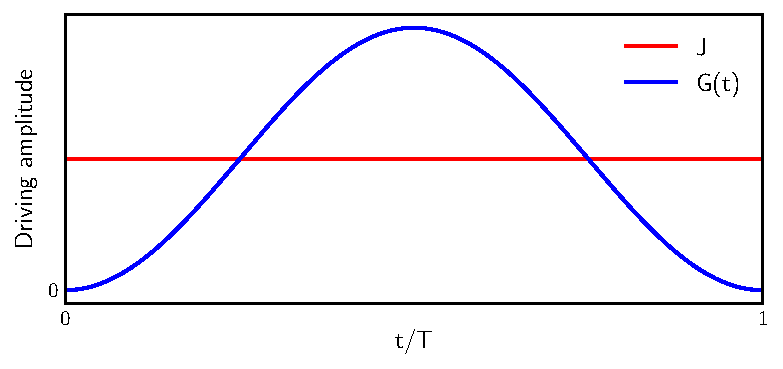
\includegraphics[width=0.5\textwidth]{continuous_flip_drive.pdf}
    \caption{Continuous spin flip drive protocol with $g_0 = \frac{\omega}{2}$. The transverse field $G(t)$ varies smoothly over time, inducing continuous spin flips.}
\end{figure}
The amplitude $g_0$ is chosen such that $\displaystyle \int_0^T G(t)\,dt = \frac{\pi}{2}$, ensuring that the transverse field induces a spin flip over one period $T = \frac{2\pi}{\omega}$. Consequently, the system is anticipated to exhibit a subharmonic response with a period of $2T$.

Explicitly,
\begin{align*}
    &\int_0^T G(t)\,dt = \frac{\pi}{2} \\
    &\int_0^T g_0\sin^2\left(\frac{\omega}{2}t \right) dt = \frac{\pi}{2}\\
    &g_0 \frac{\pi}{\omega} = \frac{\pi}{2}\\
    &\boxed{g_0 = \frac{\omega}{2}}
\end{align*}
 



We consider the spin system initially in a fully up-polarized state, such that, $\displaystyle\ket{\psi(0)} = \ket{\uparrow\uparrow\uparrow\ldots\uparrow}$. The time evolution is governed by the time-ordered exponential of the total Hamiltonian:
\begin{equation}
    \ket{\psi(t)} = \mathcal{T} \exp\left(-i\int_0^t \hat{\mathcal{H}}_{\text{total}}(t')\,dt'\right) \ket{\psi(0)}.
\end{equation}

To probe the system's dynamics, we numerically compute the expectation value of the local magnetization along the $z$-axis at each site $j$:
\begin{equation}
    m_j^z(t) = \bra{\psi(t)} \hat{\sigma}_j^z \ket{\psi(t)}.
\end{equation}  
In alignment with experimental reports~\cite{Zhang2017}, the Ising interaction strength is set to $J = 0.2/T$ for the primary set of results. To achieve a comprehensive understanding of the system's behavior under this driving protocol, we further explore a range of interaction strengths, $J \in [0.072/T, 1, 2, 10]$. The drive frequency is chosen as $\omega = 20$, which yields $g_0 = 10$.

For various interaction strengths, we numerically evaluate the magnetization dynamics and perform a Fourier transform (FFT) of the temporal magnetization data. The results are presented in the following pages.

\newpage
\subsection{$\epsilon_r = 0, J = 0.2/T, g_0 = 10, \omega = 20$}
\begin{figure}[h!]
    \centering
    \begin{minipage}[t]{0.48\textwidth}
        \centering
        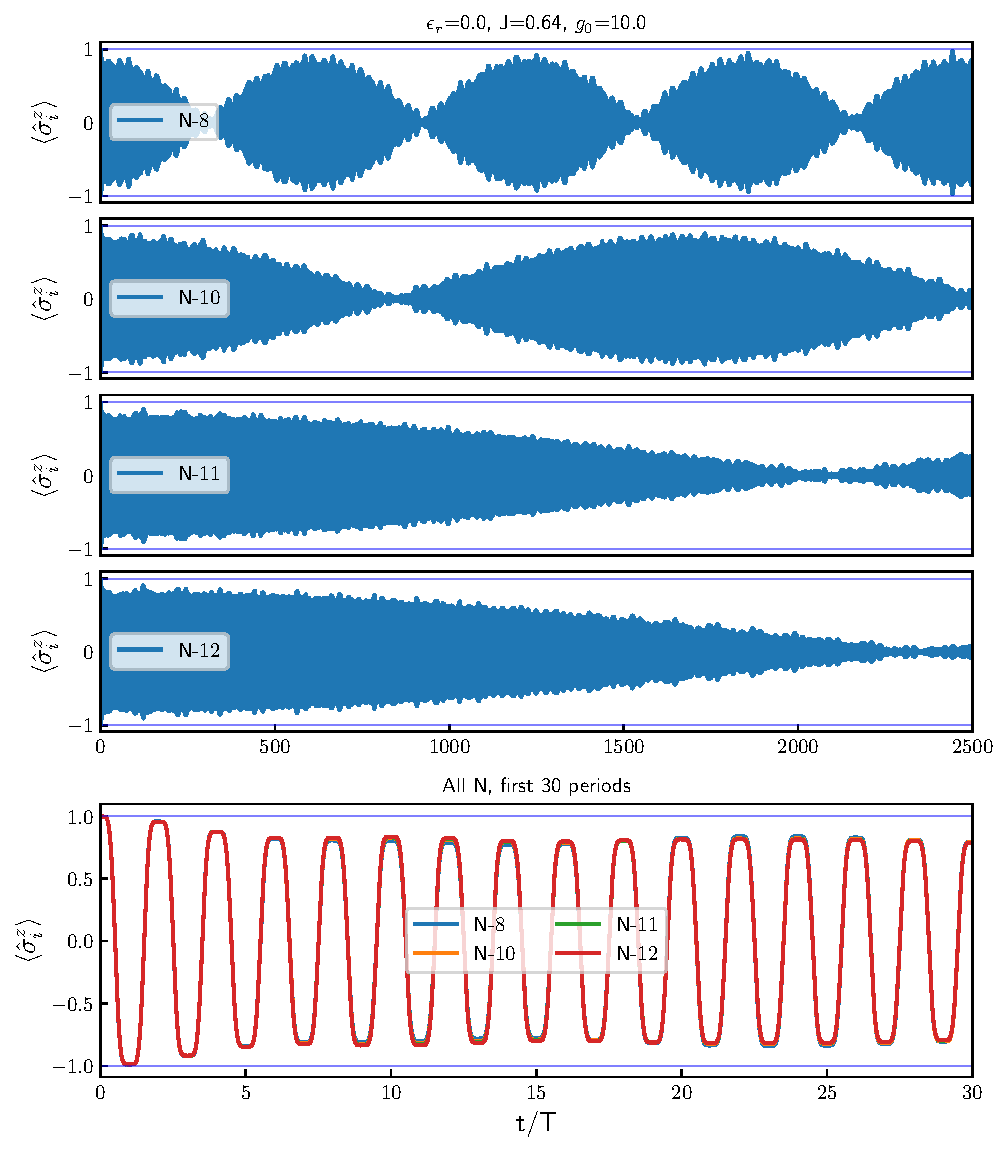
\includegraphics[width=\textwidth]{time_mag_epsilon_r0.00_J0.64_g10.0_allN.pdf}
        \caption*{(a) Magnetization dynamics for $J = 0.2/T$.}
    \end{minipage}
    \hfill
    \begin{minipage}[t]{0.48\textwidth}
        \centering
        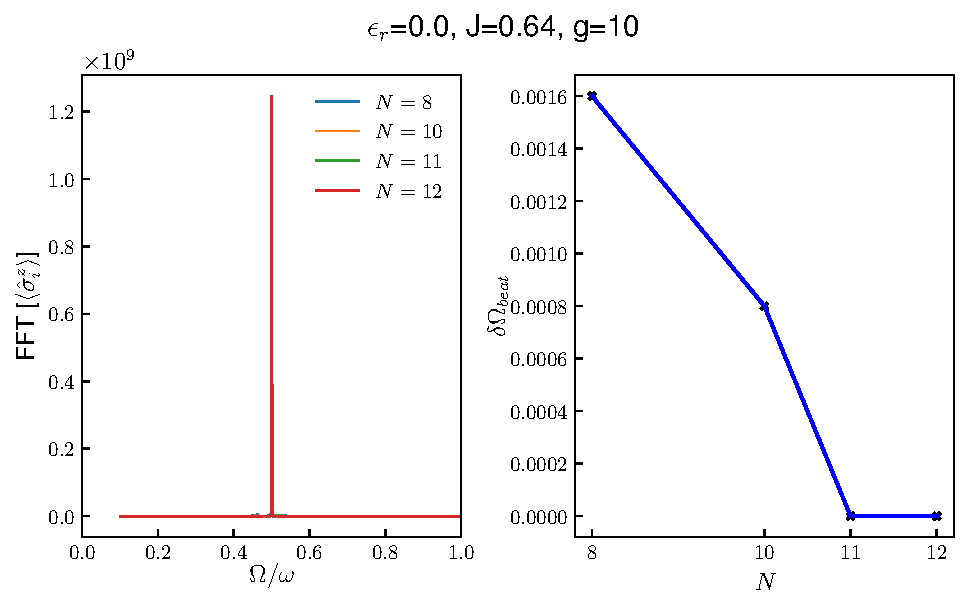
\includegraphics[width=\textwidth]{DTC_mag_fft_beat_er=0.0_J=0.6366197723675814_g=10.0.pdf}
        \caption*{(b) FFT of magnetization showing period-doubling and fall of beat frequency with system size inverse proportionality.}
    \end{minipage}
    \caption{(a) Magnetization dynamics and (b) its Fourier transform for $J = 0.2/T$. The system exhibits robust period-doubling behavior, indicative of discrete time crystal (DTC) order. The FFT reveals a pronounced peak at half the driving frequency, confirming the subharmonic response characteristic of DTCs. The beat frequency diminishes with increasing system size, suggesting enhanced stability of the DTC phase in larger systems.}
\end{figure}

The figure above illustrates the magnetization dynamics and its Fourier transform for a one-dimensional spin chain subjected to a continuous spin flip drive protocol with an interaction strength of $J = 0.2/T$. The left panel (a) displays the time evolution of the local magnetization along the $z$-axis, revealing a clear period-doubling behavior. This indicates that the system's response occurs at twice the period of the driving field, a hallmark of discrete time crystal (DTC) order. The right panel (b) presents the Fast Fourier Transform (FFT) of the magnetization data, which shows a pronounced peak at half the driving frequency. This peak confirms the subharmonic response characteristic of DTCs. Additionally, the FFT analysis indicates that the beat frequency decreases as the system size increases, suggesting that the DTC phase becomes more stable in the thermodynamic limit. Overall, these results demonstrate the emergence of DTC order in the spin chain under the specified driving conditions.

\newpage
\subsection{$\epsilon_r = 0.03, J = 0.2/T, g_0 = 10, \omega = 20$}
\begin{figure}[h!]
    \centering
    \begin{minipage}[t]{0.48\textwidth}
        \centering
        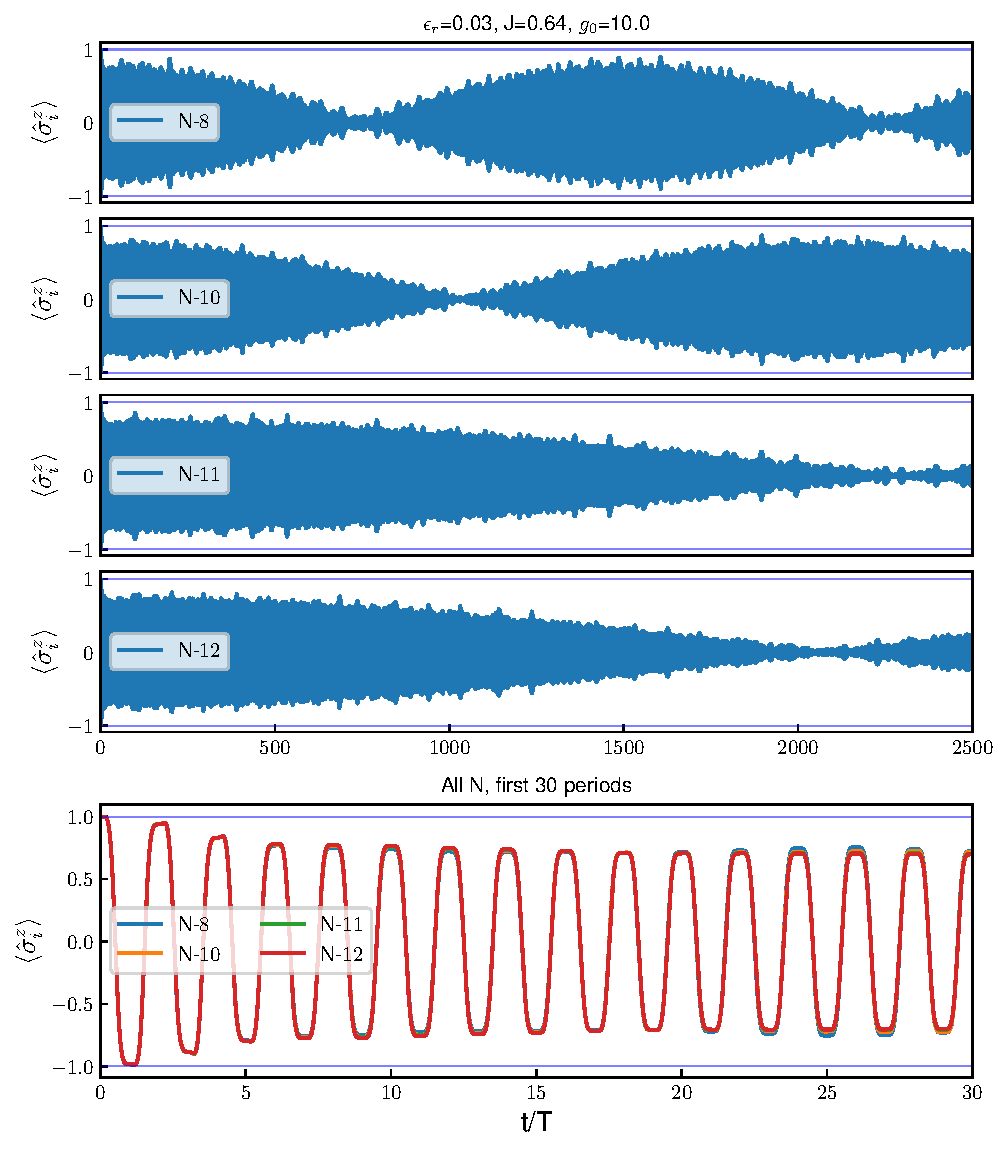
\includegraphics[width=\textwidth]{time_mag_epsilon_r0.03_J0.64_g10.0_allN.pdf}
        \caption*{(a) Magnetization dynamics for $J = 0.2/T$.}
    \end{minipage}
    \hfill
    \begin{minipage}[t]{0.48\textwidth}
        \centering
        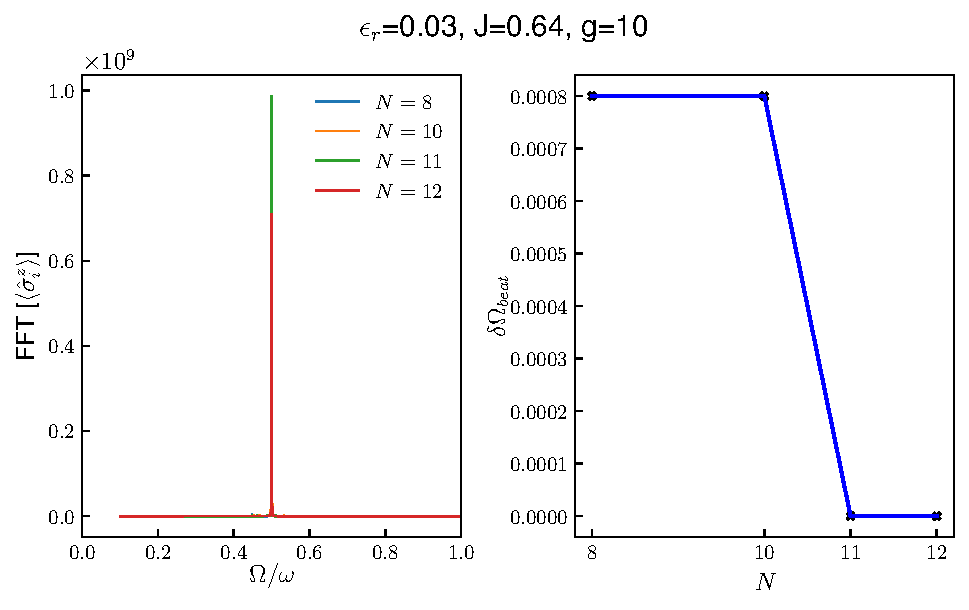
\includegraphics[width=\textwidth]{DTC_mag_fft_beat_er=0.03_J=0.6366197723675814_g=10.0.pdf}
        \caption*{(b) FFT of magnetization showing period-doubling and fall of beat frequency with system size inverse proportionality.}
    \end{minipage}
    \caption{(a) Magnetization dynamics and (b) its Fourier transform for $J = 0.2/T$. The system exhibits robust period-doubling behavior, indicative of discrete time crystal (DTC) order. The FFT reveals a pronounced peak at half the driving frequency, confirming the subharmonic response characteristic of DTCs. The beat frequency diminishes with increasing system size, suggesting enhanced stability of the DTC phase in larger systems.}
\end{figure}
\newpage
\subsection{$\epsilon_r = 0.03, J = 2, g_0 = 10, \omega = 20$}
\begin{figure}[h!]
    \centering
    \begin{minipage}[t]{0.48\textwidth} 
        \centering
        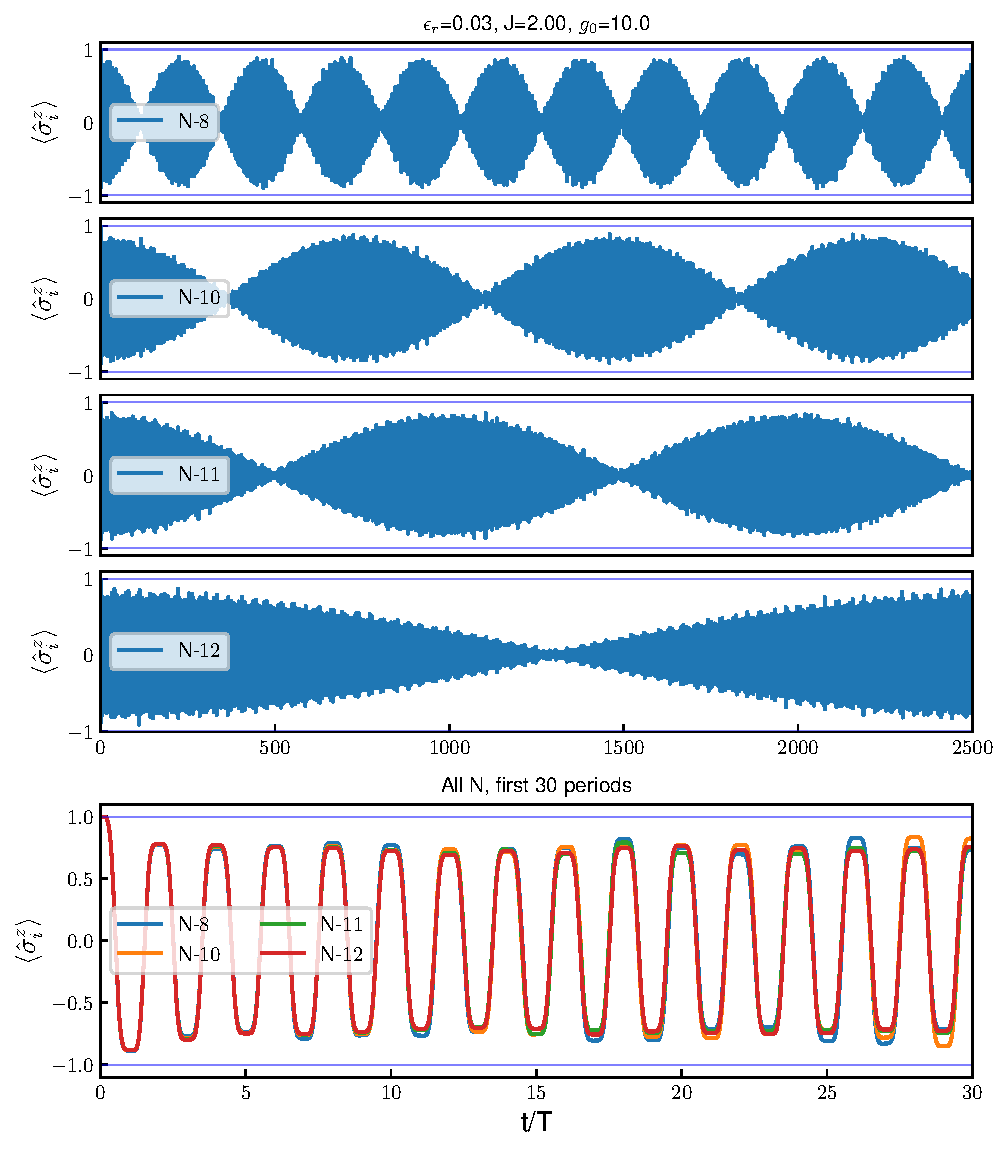
\includegraphics[width=\textwidth]{time_mag_epsilon_r0.03_J2.00_g10.0_allN.pdf}
        \caption*{(a) Magnetization dynamics for $J = 2$.}
    \end{minipage}
    \hfill
    \begin{minipage}[t]{0.48\textwidth}
        \centering
        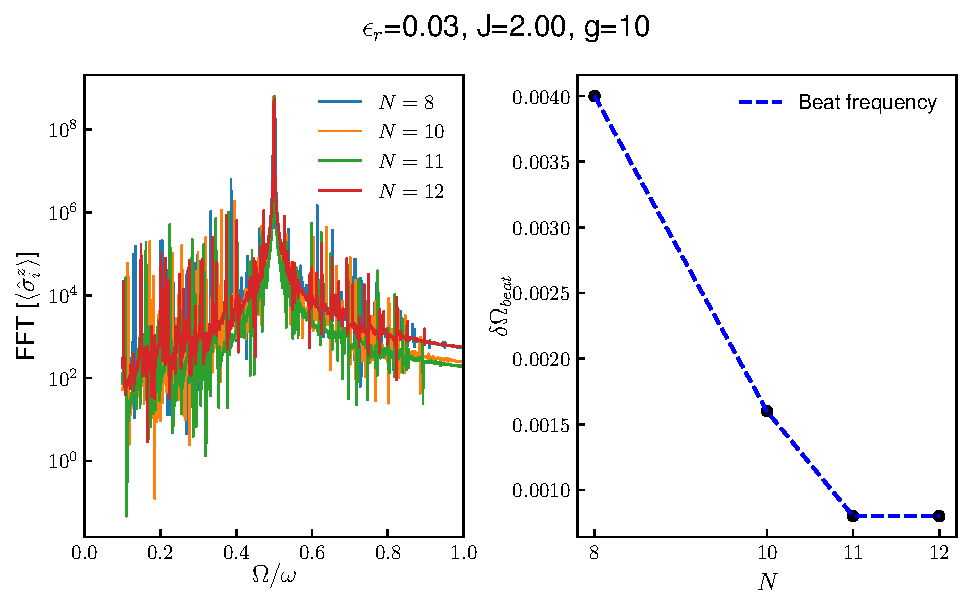
\includegraphics[width=\textwidth]{DTC_mag_fft_beat_er=0.03_J=2_g=10.0.pdf}
        \caption*{(b) FFT of magnetization showing period-doubling and fall of beat frequency with system size inverse proportionality.}
    \end{minipage}
    \caption{(a) Magnetization dynamics and (b) its Fourier transform for $J = 2$. The system exhibits robust period-doubling behavior, indicative of discrete time crystal (DTC) order. The FFT reveals a pronounced peak at half the driving frequency, confirming the    subharmonic response characteristic of DTCs. The beat frequency diminishes with increasing system size, suggesting enhanced stability of the DTC phase in larger systems.}  

\end{figure}

\newpage
\subsection{$\epsilon_r = 0.03, J = 10, g_0 = 10, \omega = 20$}
\begin{figure}[h!]
    \centering
    \begin{minipage}[t]{0.48\textwidth}     
        \centering
        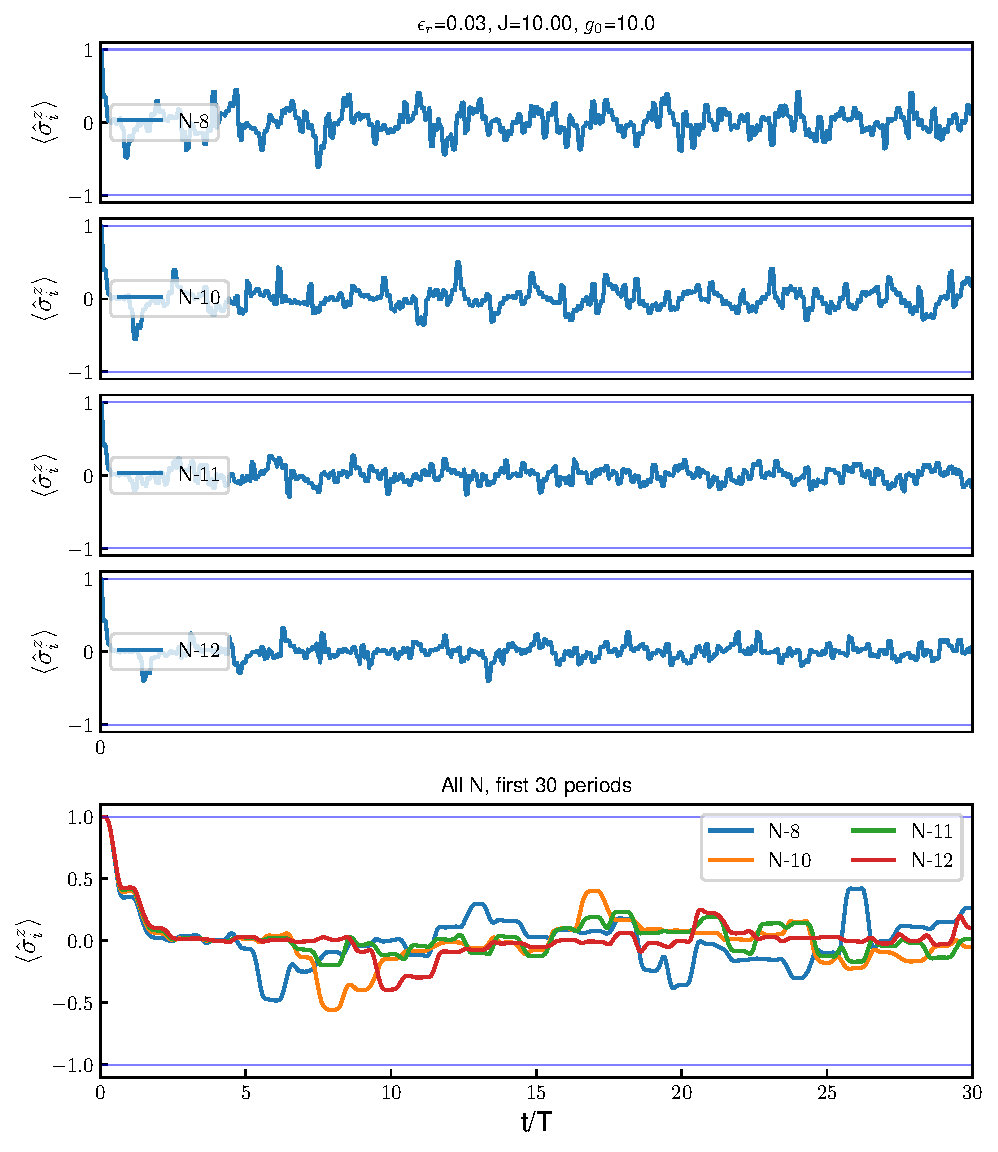
\includegraphics[width=\textwidth]{time_mag_epsilon_r0.03_J10.00_g10.0_allN.pdf}
        \caption*{(a) Magnetization dynamics for $J = 10$.}
    \end{minipage}
    \hfill
    \begin{minipage}[t]{0.48\textwidth}
        \centering
        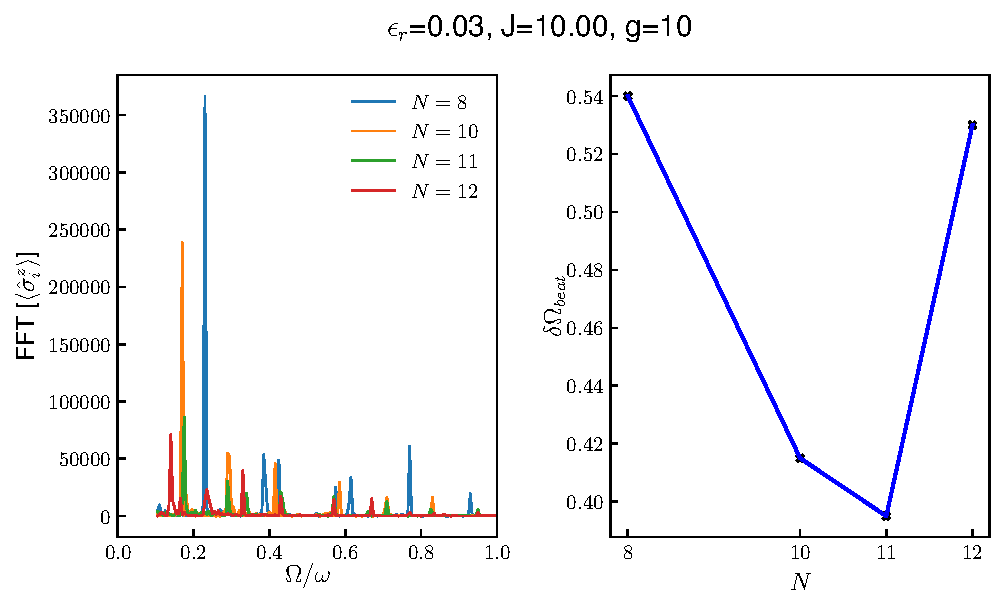
\includegraphics[width=\textwidth]{DTC_mag_fft_beat_er=0.03_J=10.0_g=10.0.pdf}
        \caption*{(b) FFT of magnetization showing period-doubling and fall of beat frequency with system size inverse proportionality.}
    \end{minipage}
    \caption{(a) Magnetization dynamics and (b) its Fourier transform for $J = 10$. The system exhibits robust period-doubling behavior, indicative of discrete time crystal (DTC) order. The FFT reveals a pronounced peak at half the driving frequency, confirming the subharmonic response characteristic of DTCs. The beat frequency diminishes with increasing system size, suggesting enhanced stability of the DTC phase in larger systems.}  
\end{figure}

\section{Conclusion}

In summary, we have investigated the emergence of discrete time crystal (DTC) order in a one-dimensional spin-$1/2$ chain subjected to a continuous spin flip drive protocol in presence of a constant nearest-neighbor spin-spin interaction. By numerically simulating the magnetization dynamics and performing Fourier analysis, we observed robust period-doubling behavior across various interaction strengths, including $J = 0.2/T$, $J = 2$ for both in presence and absence of the rotational error in the spin flip operation. The FFT results consistently revealed pronounced peaks at half the driving frequency, confirming the subharmonic response characteristic of DTCs. Notably, the beat frequency diminished with increasing system size, indicating enhanced stability of the DTC phase in the thermodynamic limit. These findings demonstrate that continuous driving can effectively stabilize DTC order, providing new insights into non-equilibrium phases of matter and their potential applications in quantum information processing.


\printbibliography
\end{document}